% cSpell:disable

% ============================================================================
% BU thesis class -- do not touch. This file carries the margins, spacing,
% title/copyright/approval/abstract page layouts and page numbering that BU
% Mugar Library requires. It has already passed a BU format review.
% ============================================================================
\usepackage{style/buthesis}

\usepackage[T1]{fontenc}
\usepackage[utf8]{inputenc}
\usepackage[english]{babel}

% Loaded explicitly: buthesis.sty only pulls in setspace, and these two used
% to arrive indirectly through the cryptography packages that were removed.
\usepackage{etoolbox}
\usepackage{ifthen}

% Uncomment to draw a frame showing the text block while checking margins:
% \usepackage[showframe]{geometry}

% ---------------------------------------------------------------- graphics --
\usepackage[usenames,dvipsnames]{xcolor}
\usepackage{graphicx}
\usepackage{subcaption}
\usepackage{adjustbox}
\usepackage{rotating}
\usepackage[final]{pdfpages}

% ------------------------------------------------------------------ tables --
\usepackage{booktabs}
\usepackage{multirow}
\usepackage{longtable}
\usepackage{makecell}
\usepackage{threeparttable}
\usepackage{colortbl}
\usepackage{array}
\usepackage{diagbox}

% ------------------------------------------------------------------- maths --
\usepackage{amsmath}
\usepackage{amsfonts}
\usepackage{amsthm}
\usepackage{mathtools}
\usepackage{nicefrac}
\usepackage{bm}
\usepackage[mathscr]{eucal}

% units and numbers -- indispensable for a methods chapter
\usepackage{siunitx}
\sisetup{
	group-minimum-digits = 4,
	per-mode             = symbol,
	range-units          = single,
	separate-uncertainty = true,
	detect-weight        = true
}
% Convenience units used throughout the methods chapter.
% siunitx does not define time units longer than a day, nor these shorthands.
\DeclareSIUnit{\molar}{M}
\DeclareSIUnit{\Molar}{\textsc{m}}
\DeclareSIUnit{\pixel}{px}
\DeclareSIUnit{\frame}{frame}
\DeclareSIUnit{\week}{week}
\DeclareSIUnit{\month}{month}
\DeclareSIUnit{\year}{year}
\DeclareSIUnit{\cell}{cell}
\DeclareSIUnit{\trial}{trial}

% ----------------------------------------------------------------- layout ---
\usepackage{appendix}
\usepackage{calc}
\usepackage{textcomp}
\usepackage{caption}
\usepackage[all]{nowidow}
% [htt] lets \texttt{} hyphenate. Without it, long monospace strings such as
% file paths and column names cannot break and run past the 1in right margin,
% which BU guide 1.1.3 forbids.
\usepackage[htt]{hyphenat}
\usepackage[inline]{enumitem}
\usepackage{soul}

% Allow TeX a little extra slack on the last resort pass rather than letting a
% line overrun the right margin by a few points. Margin compliance matters more
% than perfectly even inter-word spacing on the occasional line.
\setlength{\emergencystretch}{2em}

\PassOptionsToPackage{hyphens}{url}

% ------------------------------------------------------------------ colors --
\definecolor{BrightRed}{RGB}{204, 0, 0}
\definecolor{DarkRed}{RGB}{102, 0, 0}
\definecolor{DarkerRed}{RGB}{78, 0, 0}
\definecolor{MidRed}{RGB}{143, 0, 0}
\definecolor{lightGrey}{RGB}{220,220,220}

% Matplotlib default cycle, handy for keeping figures and text consistent.
\definecolor{MatplotlibOne}{HTML}{1F77B4}
\definecolor{MatplotlibTwo}{HTML}{FF7F0E}
\definecolor{MatplotlibThree}{HTML}{2CA02C}
\definecolor{MatplotlibFour}{HTML}{D62728}
\definecolor{MatplotlibFive}{HTML}{9467BD}
\definecolor{MatplotlibSix}{HTML}{8C564B}
\definecolor{MatplotlibSeven}{HTML}{E377C2}
\definecolor{MatplotlibEight}{HTML}{7F7F7F}
\definecolor{MatplotlibNine}{HTML}{BCBD22}
\definecolor{MatplotlibTen}{HTML}{17BECF}

% --------------------------------------------------------------- crossrefs --
% NOTE: for the copy you submit to ProQuest you may prefer black links.
% Set colorlinks=false, or linkcolor/citecolor/urlcolor to black.
\usepackage[
	colorlinks = true,
	linkcolor  = DarkRed,
	urlcolor   = MidRed,
	citecolor  = BrightRed,
]{hyperref}
\usepackage[noabbrev,capitalise]{cleveref} % must load after hyperref

\AtBeginEnvironment{appendices}{\crefalias{chapter}{appendix}}

% ------------------------------------------------------------ bibliography --
% csquotes is required by biblatex for correct quotation handling.
\usepackage{csquotes}

% BU guide 1.8.1: arrange alphabetically by the surname of the primary author,
% OR number citations in order of appearance. Do not mix the two.
% Life-science convention is author-year, which is what is configured here.
% To switch to numeric (Nature / Cell style), use:
%     style=numeric-comp, sorting=none
\usepackage[
	backend      = biber,
	style        = authoryear,
	sorting      = nyt,
	maxcitenames = 2,
	maxbibnames  = 99,
	giveninits   = true,
	uniquename   = init,
	dashed       = false,
	natbib       = true
]{biblatex}

\bibliography{bibfile}

% \printbibliography issues a \chapter*, which report.cls follows with
% \thispagestyle{plain} -- that would drop the page number to the bottom of the
% first bibliography page while every other page of the main text numbers at the
% top. BU guide 1.1.5 says to pick ONE placement for the Arabic pages, so force
% the running style back. This mirrors the \thispagestyle{myheadings} that each
% chapter file carries after its \chapter command.
\defbibheading{buchapter}[Bibliography]{%
	\chapter*{#1}%
	\thispagestyle{myheadings}%
}

% Highlight your own name in the bibliography with
%   author = {Bogatova, Daria+{highlight}} ... see biblatex annotations
\renewcommand*{\mkbibnamegiven}[1]{%
	\ifitemannotation{highlight}{\textbf{#1}}{#1}
}
\renewcommand*{\mkbibnamefamily}[1]{%
	\ifitemannotation{highlight}{\textbf{#1}}{#1}
}

\graphicspath{{./graphics/}}

\ifdefined\draft%
	\usepackage{epstopdf}
	\epstopdfDeclareGraphicsRule{.pdf}{png}{.png}{convert #1 \OutputFile}
	\DeclareGraphicsExtensions{.png,.pdf}
\fi

% --------------------------------------------------------- abbreviations ----
% BU guide 1.1.7: the List of Abbreviations must be alphabetical, NOT in order
% of appearance. The glossaries package sorts alphabetically for us.
\usepackage[
	acronym,
	nonumberlist,
	nopostdot,
	nogroupskip
]{glossaries}
% Let the abbreviations list start its own page, so no blank numbered page is
% produced. BU guide 1.1.4 forbids blank enumerated pages.
\renewcommand*{\acronymname}{List of Abbreviations}

\newglossarystyle{gloTable}
{%
	\newlength\aglslong%
	\settowidth\aglslong{\widthof{\textbf{BOLD-LONGEST}}}

	\newlength\aglsleft%
	\setlength{\aglsleft}{\dimexpr\aglslong+0.1em\relax}

	\newlength\aglsright%
	\setlength{\aglsright}{\widthof{blood oxygenation level dependent contrast}}

	\newlength\aglscenter%
	\setlength{\aglscenter}{\dimexpr\linewidth-\aglsright-\aglsleft\relax}

	\renewenvironment{theglossary}%
	{
		\begin{center}
			\begin{longtable}{
				>{\raggedright}p{\aglsleft}
				p{\aglscenter}
				>{\raggedright}p{\aglsright}
			}
	}%
	{
			\end{longtable}
		\end{center}
	}%
	\renewcommand*{\glsgroupheading}[1]{}%
	\renewcommand{\glossentry}[2]{%
		\glsentryitem{##1}\glstarget{##1}{\textbf{\glossentryname{##1}}} & \dotfill & \glossentrydesc{##1} \tabularnewline%
	}%
	\renewcommand{\subglossentry}[3]{\glossentry{##2}{##3}}%
	\ifglsnogroupskip%
		\renewcommand*{\glsgroupskip}{}%
	\else
		\renewcommand*{\glsgroupskip}{ & & \tabularnewline}%
	\fi
}
\setglossarystyle{gloTable}

\makeglossaries%

\renewcommand*{\glstextformat}[1]{\textcolor{DarkerRed}{#1}}

% ------------------------------------------------------------- theorems -----
% Rarely needed in a life-science thesis, but harmless to keep available.
\newtheorem{definition}{Definition}[section]
\newtheorem{remark}{Remark}[section]
\newtheorem{theorem}{Theorem}[section]
\newtheorem{lemma}[theorem]{Lemma}
\newtheorem{proposition}[theorem]{Proposition}
\newtheorem{corollary}[theorem]{Corollary}
\newtheorem{observation}[theorem]{Observation}
\newtheorem{example}[theorem]{Example}

% ------------------------------------------------------- drafting notes -----
% \needsinput{...} marks a place where the text needs your judgement -- a
% physical or biological rationale, a number you have to look up, or a claim
% that should not be made until it is checked. It renders as a visible,
% clearly-marked block so nothing slips into the submitted draft unnoticed.
%
% To hide every note (e.g. for the copy you send to grsrec@bu.edu), build with:
%     INTERACTION=nonstopmode pdflatex "\def\finaldraft{}% cSpell:disable

\documentclass[12pt,letterpaper]{report}

\input{version}

% cSpell:disable

% ============================================================================
% BU thesis class -- do not touch. This file carries the margins, spacing,
% title/copyright/approval/abstract page layouts and page numbering that BU
% Mugar Library requires. It has already passed a BU format review.
% ============================================================================
\usepackage{style/buthesis}

\usepackage[T1]{fontenc}
\usepackage[utf8]{inputenc}
\usepackage[english]{babel}

% Loaded explicitly: buthesis.sty only pulls in setspace, and these two used
% to arrive indirectly through the cryptography packages that were removed.
\usepackage{etoolbox}
\usepackage{ifthen}

% Uncomment to draw a frame showing the text block while checking margins:
% \usepackage[showframe]{geometry}

% ---------------------------------------------------------------- graphics --
\usepackage[usenames,dvipsnames]{xcolor}
\usepackage{graphicx}
\usepackage{subcaption}
\usepackage{adjustbox}
\usepackage{rotating}
\usepackage[final]{pdfpages}

% ------------------------------------------------------------------ tables --
\usepackage{booktabs}
\usepackage{multirow}
\usepackage{longtable}
\usepackage{makecell}
\usepackage{threeparttable}
\usepackage{colortbl}
\usepackage{array}
\usepackage{diagbox}

% ------------------------------------------------------------------- maths --
\usepackage{amsmath}
\usepackage{amsfonts}
\usepackage{amsthm}
\usepackage{mathtools}
\usepackage{nicefrac}
\usepackage{bm}
\usepackage[mathscr]{eucal}

% units and numbers -- indispensable for a methods chapter
\usepackage{siunitx}
\sisetup{
	group-minimum-digits = 4,
	per-mode             = symbol,
	range-units          = single,
	separate-uncertainty = true,
	detect-weight        = true
}
% Convenience units used throughout the methods chapter.
% siunitx does not define time units longer than a day, nor these shorthands.
\DeclareSIUnit{\molar}{M}
\DeclareSIUnit{\Molar}{\textsc{m}}
\DeclareSIUnit{\pixel}{px}
\DeclareSIUnit{\frame}{frame}
\DeclareSIUnit{\week}{week}
\DeclareSIUnit{\month}{month}
\DeclareSIUnit{\year}{year}
\DeclareSIUnit{\cell}{cell}
\DeclareSIUnit{\trial}{trial}

% ----------------------------------------------------------------- layout ---
\usepackage{appendix}
\usepackage{calc}
\usepackage{textcomp}
\usepackage{caption}
\usepackage[all]{nowidow}
% [htt] lets \texttt{} hyphenate. Without it, long monospace strings such as
% file paths and column names cannot break and run past the 1in right margin,
% which BU guide 1.1.3 forbids.
\usepackage[htt]{hyphenat}
\usepackage[inline]{enumitem}
\usepackage{soul}

% Allow TeX a little extra slack on the last resort pass rather than letting a
% line overrun the right margin by a few points. Margin compliance matters more
% than perfectly even inter-word spacing on the occasional line.
\setlength{\emergencystretch}{2em}

\PassOptionsToPackage{hyphens}{url}

% ------------------------------------------------------------------ colors --
\definecolor{BrightRed}{RGB}{204, 0, 0}
\definecolor{DarkRed}{RGB}{102, 0, 0}
\definecolor{DarkerRed}{RGB}{78, 0, 0}
\definecolor{MidRed}{RGB}{143, 0, 0}
\definecolor{lightGrey}{RGB}{220,220,220}

% Matplotlib default cycle, handy for keeping figures and text consistent.
\definecolor{MatplotlibOne}{HTML}{1F77B4}
\definecolor{MatplotlibTwo}{HTML}{FF7F0E}
\definecolor{MatplotlibThree}{HTML}{2CA02C}
\definecolor{MatplotlibFour}{HTML}{D62728}
\definecolor{MatplotlibFive}{HTML}{9467BD}
\definecolor{MatplotlibSix}{HTML}{8C564B}
\definecolor{MatplotlibSeven}{HTML}{E377C2}
\definecolor{MatplotlibEight}{HTML}{7F7F7F}
\definecolor{MatplotlibNine}{HTML}{BCBD22}
\definecolor{MatplotlibTen}{HTML}{17BECF}

% --------------------------------------------------------------- crossrefs --
% NOTE: for the copy you submit to ProQuest you may prefer black links.
% Set colorlinks=false, or linkcolor/citecolor/urlcolor to black.
\usepackage[
	colorlinks = true,
	linkcolor  = DarkRed,
	urlcolor   = MidRed,
	citecolor  = BrightRed,
]{hyperref}
\usepackage[noabbrev,capitalise]{cleveref} % must load after hyperref

\AtBeginEnvironment{appendices}{\crefalias{chapter}{appendix}}

% ------------------------------------------------------------ bibliography --
% csquotes is required by biblatex for correct quotation handling.
\usepackage{csquotes}

% BU guide 1.8.1: arrange alphabetically by the surname of the primary author,
% OR number citations in order of appearance. Do not mix the two.
% Life-science convention is author-year, which is what is configured here.
% To switch to numeric (Nature / Cell style), use:
%     style=numeric-comp, sorting=none
\usepackage[
	backend      = biber,
	style        = authoryear,
	sorting      = nyt,
	maxcitenames = 2,
	maxbibnames  = 99,
	giveninits   = true,
	uniquename   = init,
	dashed       = false,
	natbib       = true
]{biblatex}

\bibliography{bibfile}

% \printbibliography issues a \chapter*, which report.cls follows with
% \thispagestyle{plain} -- that would drop the page number to the bottom of the
% first bibliography page while every other page of the main text numbers at the
% top. BU guide 1.1.5 says to pick ONE placement for the Arabic pages, so force
% the running style back. This mirrors the \thispagestyle{myheadings} that each
% chapter file carries after its \chapter command.
\defbibheading{buchapter}[Bibliography]{%
	\chapter*{#1}%
	\thispagestyle{myheadings}%
}

% Highlight your own name in the bibliography with
%   author = {Bogatova, Daria+{highlight}} ... see biblatex annotations
\renewcommand*{\mkbibnamegiven}[1]{%
	\ifitemannotation{highlight}{\textbf{#1}}{#1}
}
\renewcommand*{\mkbibnamefamily}[1]{%
	\ifitemannotation{highlight}{\textbf{#1}}{#1}
}

\graphicspath{{./graphics/}}

\ifdefined\draft%
	\usepackage{epstopdf}
	\epstopdfDeclareGraphicsRule{.pdf}{png}{.png}{convert #1 \OutputFile}
	\DeclareGraphicsExtensions{.png,.pdf}
\fi

% --------------------------------------------------------- abbreviations ----
% BU guide 1.1.7: the List of Abbreviations must be alphabetical, NOT in order
% of appearance. The glossaries package sorts alphabetically for us.
\usepackage[
	acronym,
	nonumberlist,
	nopostdot,
	nogroupskip
]{glossaries}
% Let the abbreviations list start its own page, so no blank numbered page is
% produced. BU guide 1.1.4 forbids blank enumerated pages.
\renewcommand*{\acronymname}{List of Abbreviations}

\newglossarystyle{gloTable}
{%
	\newlength\aglslong%
	\settowidth\aglslong{\widthof{\textbf{BOLD-LONGEST}}}

	\newlength\aglsleft%
	\setlength{\aglsleft}{\dimexpr\aglslong+0.1em\relax}

	\newlength\aglsright%
	\setlength{\aglsright}{\widthof{blood oxygenation level dependent contrast}}

	\newlength\aglscenter%
	\setlength{\aglscenter}{\dimexpr\linewidth-\aglsright-\aglsleft\relax}

	\renewenvironment{theglossary}%
	{
		\begin{center}
			\begin{longtable}{
				>{\raggedright}p{\aglsleft}
				p{\aglscenter}
				>{\raggedright}p{\aglsright}
			}
	}%
	{
			\end{longtable}
		\end{center}
	}%
	\renewcommand*{\glsgroupheading}[1]{}%
	\renewcommand{\glossentry}[2]{%
		\glsentryitem{##1}\glstarget{##1}{\textbf{\glossentryname{##1}}} & \dotfill & \glossentrydesc{##1} \tabularnewline%
	}%
	\renewcommand{\subglossentry}[3]{\glossentry{##2}{##3}}%
	\ifglsnogroupskip%
		\renewcommand*{\glsgroupskip}{}%
	\else
		\renewcommand*{\glsgroupskip}{ & & \tabularnewline}%
	\fi
}
\setglossarystyle{gloTable}

\makeglossaries%

\renewcommand*{\glstextformat}[1]{\textcolor{DarkerRed}{#1}}

% ------------------------------------------------------------- theorems -----
% Rarely needed in a life-science thesis, but harmless to keep available.
\newtheorem{definition}{Definition}[section]
\newtheorem{remark}{Remark}[section]
\newtheorem{theorem}{Theorem}[section]
\newtheorem{lemma}[theorem]{Lemma}
\newtheorem{proposition}[theorem]{Proposition}
\newtheorem{corollary}[theorem]{Corollary}
\newtheorem{observation}[theorem]{Observation}
\newtheorem{example}[theorem]{Example}

% ------------------------------------------------------- drafting notes -----
% \needsinput{...} marks a place where the text needs your judgement -- a
% physical or biological rationale, a number you have to look up, or a claim
% that should not be made until it is checked. It renders as a visible,
% clearly-marked block so nothing slips into the submitted draft unnoticed.
%
% To hide every note (e.g. for the copy you send to grsrec@bu.edu), build with:
%     INTERACTION=nonstopmode pdflatex "\def\finaldraft{}% cSpell:disable

\documentclass[12pt,letterpaper]{report}

\input{version}

\input{preamble}

\input{glossary}

\begin{document}

	% ========================================================================
	% PRELIMINARY PAGES
	%
	% BU guide 1.1.6 fixes this order and this pagination:
	%   Title page              i    (counted, number not printed)
	%   Copyright page          ii   (counted, number not printed)
	%   Readers' approval page  iii  (counted, number not printed, UNSIGNED)
	%   Dedication (optional)   iv
	%   Acknowledgments (opt.)  v
	%   Abstract (required)     vi
	%   Preface (optional)      vii
	%   Table of Contents       viii
	%   List of Tables          (required if you have any tables)
	%   List of Figures         (required if you have any figures)
	%   List of Illustrations   (required if you have any)
	%   List of Abbreviations   (alphabetical)
	%   Glossary                (if applicable)
	%   First page of text      1
	%
	% Pagination is continuous: if you omit an optional section, do not skip
	% its number, just carry on.
	% ========================================================================

	\input{meta}

	\maketitle%
	\cleardoublepage%

	\copyrightpage%
	\cleardoublepage%

	\approvalpage%
	\cleardoublepage%

	% Dedication
	%\IfFileExists%
	%	{frontmatter/dedication.tex}
	%	{
	%		\ifx\noAcks\undefined%
	%			\newpage
	%			\phantomsection%
	%			\addcontentsline{toc}{chapter}{Dedication}
	%			\input{frontmatter/dedication}
	%			\cleardoublepage%
	%		\fi
	%	}
	%	{}

	% Acknowledgments
	%\IfFileExists%
	%	{frontmatter/acknowledgments.tex}
	%	{
	%		\ifx\noAcks\undefined%
	%			\newpage
	%			\phantomsection%
	%			\addcontentsline{toc}{chapter}{Acknowledgments}
	%			\input{frontmatter/acknowledgments}
	%			\cleardoublepage%
	%		\fi
	%	}
	%	{}

	% Abstract -- required. \abstractpage prints the title / author / school /
	% major professor header that BU requires above the word ABSTRACT.
	\phantomsection%
	\addcontentsline{toc}{chapter}{Abstract}
	\begin{abstractpage}
		\input{frontmatter/abstract}
	\end{abstractpage}
	\cleardoublepage%

	% ------------------------------------------------------------------------
	% Table of Contents.
	% tocdepth 2 lists chapters, sections and subsections. Raise to 3 or 4 if
	% your committee wants deeper subheadings (BU guide 1.6 allows either).
	% ------------------------------------------------------------------------
	\setcounter{tocdepth}{2}
	\phantomsection%
	\addcontentsline{toc}{chapter}{Table of Contents}
	\tableofcontents
	\cleardoublepage%

	% ------------------------------------------------------------------------
	% Lists, in the order required by BU guide 1.1.6:
	% Tables, then Figures, then Illustrations, then Abbreviations.
	% Each list is REQUIRED if the document contains any of that element, and
	% must be DELETED if it does not. Comment out whichever you do not need.
	% ------------------------------------------------------------------------
	\newpage
	\phantomsection%
	\addcontentsline{toc}{chapter}{\listtablename}
	\listoftables
	\cleardoublepage%

	\newpage
	\phantomsection%
	\addcontentsline{toc}{chapter}{\listfigurename}
	\listoffigures
	\cleardoublepage%

	% List of Abbreviations -- sorted alphabetically by the glossaries package.
	% Only abbreviations actually used in the text appear here; see glossary.tex
	% if you want to force every defined entry into the list.
	\phantomsection%
	\addcontentsline{toc}{chapter}{List of Abbreviations}
	\printglossary[type=\acronymtype, title={List of Abbreviations}]
	\cleardoublepage%

	% ========================================================================
	% MAIN TEXT -- Arabic numerals restart at 1 here.
	% ========================================================================
	\newpage
	\endofprelim%
	\cleardoublepage%

	\input{sections/introduction}
	\cleardoublepage%

	\input{sections/methods}
	\cleardoublepage%

	\input{sections/study-one}
	\cleardoublepage%

	\input{sections/study-two}
	\cleardoublepage%

	\input{sections/discussion}
	\cleardoublepage%

	% ========================================================================
	% END MATTER
	% BU guide 1.1.6 and 1.7: appendices FIRST, then the bibliography, then the
	% vita last. Pagination continues in Arabic numerals throughout -- do not
	% restart or use A-1, A-2 style numbers in the appendices.
	% ========================================================================
	\begin{appendices}

		\input{endmatter/appendix-supplementary}
		\cleardoublepage%

	\end{appendices}

	% Bibliography. Single spacing with a blank line between entries is
	% explicitly allowed by BU guide 1.8.1.
	\newpage
	\singlespace%

	\phantomsection%
	\addcontentsline{toc}{chapter}{Bibliography}

	\printbibliography[heading=buchapter]

	\cleardoublepage%

	% Curriculum Vitae -- required of ALL students, and must be the last
	% numbered page(s). Keep it to three or four pages (BU guide 1.9).
	\input{endmatter/cv}

\end{document}
"
% or simply define \finaldraft at the top of main.tex.
%
% Check for leftovers before submitting:
%     grep -rn "needsinput" document/sections
\ifdefined\finaldraft%
	\newcommand{\needsinput}[1]{}
\else
	\newcommand{\needsinput}[1]{%
		\par\medskip\noindent
		\begingroup
			\small\sffamily\color{DarkRed}%
			\begin{singlespace}%
				\textbf{[NEEDS INPUT]}\quad #1%
			\end{singlespace}%
		\endgroup
		\par\medskip
	}
\fi

% -------------------------------------------------------------- shortcuts ---
% Statistics shorthands, so reporting stays consistent across chapters.
\newcommand{\pval}[1]{\ensuremath{p = #1}}
\newcommand{\pless}[1]{\ensuremath{p < #1}}
\newcommand{\mean}[2]{\ensuremath{#1 \pm #2}}
\newcommand{\nanimals}[1]{\ensuremath{n = #1}}

% Common italicised terms -- keeps species and gene names typeset correctly.
\newcommand{\invivo}{\emph{in vivo}}
\newcommand{\invitro}{\emph{in vitro}}
\newcommand{\exvivo}{\emph{ex vivo}}
\newcommand{\etal}{\emph{et al.}}

% Software names. Plain macros rather than glossary entries so they are safe to
% use inside captions and headings.
\newcommand{\mavca}{MAVCA}
\newcommand{\napari}{\textsc{napari}}

% Full citation of your own publications, used in the Introduction.
\newcommand{\printpublication}[1]{\AtNextCite{\defcounter{maxnames}{99}}\fullcite{#1}}

% ---------------------------------------------------------- approval page ---
% \readerC{ordinal}{name}{official title}{institution or empty}
%
% Always renders a blank signature rule. The copy submitted to ProQuest must be
% UNSIGNED (BU guide 1.4.1); signatures are collected through DocuSign and
% GRS attaches the signed page after review.
%
% Takes FOUR arguments. buthesis.sty's underlying \reader takes a fifth for the
% signature, which is supplied here, so you never pass it yourself. An earlier
% five-argument version silently swallowed the following token whenever a reader
% line was written with only four -- hence the fixed arity.
%
% Leave the institution empty for BU faculty. BU guide 1.4.3: a reader is
% assumed to be BU faculty unless you name another institution.
\newcommand{\readerC}[4]{%
	\reader{#1}{#2}{#3}{#4}{\rule{0.75\textwidth}{0.1mm}}%
}


% ============================================================================
% LIST OF ABBREVIATIONS
%
% BU guide 1.1.7: "If you include a List of Abbreviations, it must be arranged
% alphabetically, not by order of appearance of the abbreviation in the text."
% The glossaries package sorts alphabetically automatically, so simply add
% entries wherever is convenient.
%
% Usage in the text:
%   \acrshort{bold}   -> BOLD
%   \acrlong{bold}    -> blood oxygenation level dependent
%   \acrfull{bold}    -> blood oxygenation level dependent (BOLD)
%   \gls{bold}        -> spells it out the first time, then abbreviates
%   \acrshortpl{roi}  -> ROIs (plural)
%
% \glsaddall in preamble.tex forces every entry to appear in the list even if
% it is never cited. Delete entries you do not use, or drop \glsaddall.
%
% TODO: this is a generic neuroscience / BME starter set. Prune it and add the
% abbreviations your own chapters actually use.
% ============================================================================

% Only abbreviations you actually cite in the text (with \acrshort, \gls, etc.)
% appear in the List of Abbreviations. That is usually what you want: a list of
% abbreviations you never use would be padding. If you would rather force every
% entry below into the list, uncomment the next line.
% \glsaddall

% ------------------------------------------------------------- imaging ------
\newacronym{scape}{SCAPE}{swept confocally-aligned planar excitation microscopy}
\newacronym{mavca}{MAVCA}{Mask-Assisted Volumetric Calcium Analysis}
\newacronym{mad}{MAD}{median absolute deviation}
\newacronym{bold}{BOLD}{blood oxygenation level dependent}
\newacronym{fmri}{fMRI}{functional magnetic resonance imaging}
\newacronym{mri}{MRI}{magnetic resonance imaging}
\newacronym{oct}{OCT}{optical coherence tomography}
\newacronym{nirs}{NIRS}{near-infrared spectroscopy}
\newacronym{fnirs}{fNIRS}{functional near-infrared spectroscopy}
\newacronym{osa}{OSA}{oxygen-sensitive absorption}
\newacronym{tpm}{2PM}{two-photon microscopy}
\newacronym{tplsm}{TPLSM}{two-photon laser scanning microscopy}
\newacronym{psf}{PSF}{point spread function}
\newacronym{na}{NA}{numerical aperture}
\newacronym{fov}{FOV}{field of view}
\newacronym{snr}{SNR}{signal-to-noise ratio}
\newacronym{cbf}{CBF}{cerebral blood flow}
\newacronym{cbv}{CBV}{cerebral blood volume}
\newacronym{cmro}{CMRO\textsubscript{2}}{cerebral metabolic rate of oxygen}
\newacronym{po}{pO\textsubscript{2}}{partial pressure of oxygen}
\newacronym{so}{SO\textsubscript{2}}{oxygen saturation}
\newacronym{hbo}{HbO}{oxygenated hemoglobin}
\newacronym{hbr}{HbR}{deoxygenated hemoglobin}

% ------------------------------------------------------- indicators ---------
\newacronym{geci}{GECI}{genetically encoded calcium indicator}
\newacronym{gevi}{GEVI}{genetically encoded voltage indicator}
\newacronym{gfp}{GFP}{green fluorescent protein}
\newacronym{rfp}{RFP}{red fluorescent protein}
\newacronym{aav}{AAV}{adeno-associated virus}
\newacronym{cre}{Cre}{causes recombination recombinase}
\newacronym{dreadd}{DREADD}{designer receptor exclusively activated by designer drugs}
\newacronym{cno}{CNO}{clozapine-N-oxide}
\newacronym{chr}{ChR2}{channelrhodopsin-2}

% ----------------------------------------------------------- anatomy --------
\newacronym{cns}{CNS}{central nervous system}
\newacronym{pfc}{PFC}{prefrontal cortex}
\newacronym{sone}{S1}{primary somatosensory cortex}
\newacronym{vone}{V1}{primary visual cortex}
\newacronym{lfive}{L5}{cortical layer 5}
\newacronym{roi}{ROI}{region of interest}
\newacronym{bbb}{BBB}{blood--brain barrier}

% ------------------------------------------------------ electrophysiology ---
\newacronym{lfp}{LFP}{local field potential}
\newacronym{eeg}{EEG}{electroencephalography}
\newacronym{ecog}{ECoG}{electrocorticography}
\newacronym{epsp}{EPSP}{excitatory postsynaptic potential}
\newacronym{ipsp}{IPSP}{inhibitory postsynaptic potential}
\newacronym{ap}{AP}{action potential}

% ---------------------------------------------------------- analysis --------
\newacronym{anova}{ANOVA}{analysis of variance}
\newacronym{glm}{GLM}{general linear model}
\newacronym{lme}{LME}{linear mixed-effects model}
\newacronym{sem}{SEM}{standard error of the mean}
\newacronym{sd}{SD}{standard deviation}
\newacronym{ci}{CI}{confidence interval}
\newacronym{pca}{PCA}{principal component analysis}
\newacronym{fdr}{FDR}{false discovery rate}
\newacronym{hrf}{HRF}{hemodynamic response function}

% --------------------------------------------------------- regulatory ------
\newacronym{iacuc}{IACUC}{Institutional Animal Care and Use Committee}
\newacronym{arrive}{ARRIVE}{Animal Research: Reporting of In Vivo Experiments}
\newacronym{nih}{NIH}{National Institutes of Health}
\newacronym{bu}{BU}{Boston University}


\begin{document}

	% ========================================================================
	% PRELIMINARY PAGES
	%
	% BU guide 1.1.6 fixes this order and this pagination:
	%   Title page              i    (counted, number not printed)
	%   Copyright page          ii   (counted, number not printed)
	%   Readers' approval page  iii  (counted, number not printed, UNSIGNED)
	%   Dedication (optional)   iv
	%   Acknowledgments (opt.)  v
	%   Abstract (required)     vi
	%   Preface (optional)      vii
	%   Table of Contents       viii
	%   List of Tables          (required if you have any tables)
	%   List of Figures         (required if you have any figures)
	%   List of Illustrations   (required if you have any)
	%   List of Abbreviations   (alphabetical)
	%   Glossary                (if applicable)
	%   First page of text      1
	%
	% Pagination is continuous: if you omit an optional section, do not skip
	% its number, just carry on.
	% ========================================================================

	% cSpell:ignore pdftitle pdfsubject pdfkeywords pdfcreator pdfproducer

% ============================================================================
% TODO: Confirm the exact wording of your title with your committee.
% Taken from your CV, where it appears as both your dissertation title and a
% manuscript in preparation.
% BU guide 1.2.1: keep it brief and descriptive. Acronyms are discouraged.
% ProQuest cannot reproduce formulae, superscripts, subscripts or symbols.
% BU guide 1.2.3: do not name the discipline in the title.
% ============================================================================
\title{Behavioral-State-Dependent Calcium Dynamics in the Apical Dendrites of L5 Pyramidal Cells}
\author{Daria Bogatova}

% 1 = Master's thesis, 2 = Doctoral dissertation, 3 = both
\degree=2

% Previous degrees, one per line, oldest first.
\prevdegrees{
	B.S., Goethe University Frankfurt, 2021 \\
	M.S., Boston University, 2024
}

% ----------------------------------------------------------------------------
% Official school name for the title page. BU guide p.27 lists the only
% permitted forms. Use "Graduate School of Arts and Sciences" for a GRS
% program (e.g. the Neuroscience PhD). If you are registered in Biomedical
% Engineering, this MUST read "College of Engineering" instead.
% ----------------------------------------------------------------------------
\department{Graduate School of Arts and Sciences}

% Year the degree is officially conferred -- not the year you defend.
\defenseyear{2027}
\degreeyear{2027}

% ============================================================================
% READERS
% \readerC{ordinal}{name}{official title}{institution or empty} -- four args.
% BU guide 1.4.3: put the official title after the name ("Professor of
% Neuroscience"). Never write "Dr." before a name.
% The signature line is always rendered blank: the copy you submit must be
% UNSIGNED, and signatures are collected separately through DocuSign.
% ============================================================================
% Leave the institution (4th argument) empty for BU faculty. BU guide 1.4.3:
% a reader is assumed to be BU faculty unless you name another institution.
% Verify each official title before the DocuSign page goes out.
\readerC{First}{Anna Devor, Ph.D.}{Professor of Biomedical Engineering}{}
\readerC{Second}{Ian Davison, Ph.D.}{Professor of Biology}{}
\readerC{Third}{Michael Hasselmo, Ph.D.}{Professor of Biomedical Engineering}{}
\readerC{Fourth}{Lynne Chantranupong, Ph.D.}{Assistant Professor of Biology}{}

% Major professor shown on the abstract page. Should match the first reader.
\numadvisors=1
\majorprof{Anna Devor, Ph.D.}{Professor of Biomedical Engineering}

\hypersetup{
	pdfauthor   = {Daria Bogatova},
	pdftitle    = {Behavioral-State-Dependent Calcium Dynamics in the Apical Dendrites of L5 Pyramidal Cells},
	pdfsubject  = {Doctoral Dissertation},
	pdfkeywords = {apical dendrites, layer 5 pyramidal neurons, calcium imaging, neuromodulation, two-photon microscopy, SCAPE},
	pdfcreator  = {LaTeX with hyperref package},
	pdfproducer = {pdflatex}
}


	\maketitle%
	\cleardoublepage%

	\copyrightpage%
	\cleardoublepage%

	\approvalpage%
	\cleardoublepage%

	% Dedication
	%\IfFileExists%
	%	{frontmatter/dedication.tex}
	%	{
	%		\ifx\noAcks\undefined%
	%			\newpage
	%			\phantomsection%
	%			\addcontentsline{toc}{chapter}{Dedication}
	%			\section*{\centerline{Dedication}}

	% ------------------------------------------------------------------------
	% TODO: Write your dedication, or delete this file entirely.
	% The dedication is optional (BU guide 1.1.6) and becomes page iv.
	% main.tex skips it automatically if this file does not exist.
	% ------------------------------------------------------------------------
	I dedicate this work to \ldots

	%			\cleardoublepage%
	%		\fi
	%	}
	%	{}

	% Acknowledgments
	%\IfFileExists%
	%	{frontmatter/acknowledgments.tex}
	%	{
	%		\ifx\noAcks\undefined%
	%			\newpage
	%			\phantomsection%
	%			\addcontentsline{toc}{chapter}{Acknowledgments}
	%			\section*{\centerline{Acknowledgments}}

	Anna, everything I am professionally, and the very fact that I am here today --- I owe to you.
	You were beside me through the darkest and hardest moments of my life.
	You showed me what not giving up truly looks like: continuing to show up, staying when things became frightening, and holding hope for someone when they could no longer hold it alone.

	With you, I never had to pretend that I was stronger than I felt.
	I could rely on you, fall apart in front of you, and know that you would still see me --- not as a burden, but simply as myself.
	You never needed me to be brave for your comfort.
	You allowed me to be frightened, exhausted, and uncertain, while continuing to treat me as someone who had a future.
	When I could not see beyond the next day, you kept seeing a life ahead of me --- and a place for me in science.

	Somewhere along the way, you became far more than my advisor.
	You became my friend, and I do not use that word lightly.
	It means that I trust you with the parts of myself I usually keep hidden.
	It means that your presence has made both the joyful moments fuller and the unbearable ones survivable.

	I do not know how to thank someone for shaping my work, protecting my future, and helping me remain here to live it.
	When you look at these pages, I hope you see more than the research you helped make possible.
	I hope you see the life you continued to believe in when I could not.

	Neither this dissertation nor the person writing it would exist in the same way without you. 
	(In case I die before defense, Ayla, please delete last sentence.)

	%			\cleardoublepage%
	%		\fi
	%	}
	%	{}

	% Abstract -- required. \abstractpage prints the title / author / school /
	% major professor header that BU requires above the word ABSTRACT.
	\phantomsection%
	\addcontentsline{toc}{chapter}{Abstract}
	\begin{abstractpage}
		% ============================================================================
% ABSTRACT
% BU guide 1.5.1: the abstract must contain a clear and brief statement of
%   (1) the problem, (2) the procedures / methods followed, (3) the results,
%   and (4) the conclusions.
% There is no word limit any more, but be concise. Double spaced.
% Do NOT include graphs, charts, tables or illustrations here (guide 1.5.3).
% Include full proper nouns and place names -- the abstract is keyword
% searchable in ProQuest.
% ============================================================================

Apical dendrites of layer 5 pyramidal cells (L5PCs) are critical integrative hubs in cortical circuits. 
The repertoire of their activity patterns, including $\mathrm{Ca}^{2+}$ and NMDA spikes, varies across brain states.
However, the relationship between neuromodulatory activity and the statistical properties of dendritic $\mathrm{Ca}^{2+}$ and NMDA spikes remains unclear.
In this study, we performed volumetric imaging to characterize spontaneous $\mathrm{Ca}^{2+}$ dynamics in the apical dendrites of L5PCs in awake, head-fixed mice. 
We used Rbp4-Cre mice, retro-orbitally injected with PHP.eB AAVs to express GCaMP6s in L5PCs, and a red fluorescent acetylcholine (ACh) sensor GRAB-ACh. 
Using light sheet microscopy (SCAPE-2.0, Voleti et al. 2019) we imaged spontaneous $\mathrm{Ca}^{2+}$ and ACh activity in the primary somatosensory (SI) cortex at a volumetric rate of $\SI{5}{\hertz}$ with a $400 \times 200 \times 150 \,\mathrm{\mu m}^3$ field of view, capturing the top $\approx 150 \,\mathrm{\mu m}$.
Simultaneously, we acquired behavior readouts: the eye pupil diameter, whisking, and accelerometer-based body movement. 
Data were analyzed using a custom Python toolbox for detection and segmentation of dendritic events from volumetric time series.
Our results show high correlation between global (averaged within the volume) dendritic $\mathrm{Ca}^{2+}$ dynamics, ACh, and the behavior readouts.
Activity-dependent segmentation of dendritic regions of interest (ROIs) revealed several types of events including vertically oriented putative $\mathrm{Ca}^{2+}$ spikes engulfing the nexus and apical trunk as well as $\mathrm{Ca}^{2+}$ transients localized to specific dendritic branches (putative NMDA-dependent synaptic events).
The probability of putative $\mathrm{Ca}^{2+}$ spikes increased with an increase in ACh. 
To investigate the relationship between dendritic $\mathrm{Ca}^{2+}$ activity and somatic spiking, we used random access 2-photon microscopy (Femto3D Atlas, Femtonics). 
Our preliminary data suggest that most of the events observable within the top $\approx 150 \,\mathrm{\mu m}$ correspond to synaptic inputs and dendritic $\mathrm{Ca}^{2+}$ spikes rather than back-propagated action potentials.

	\end{abstractpage}
	\cleardoublepage%

	% ------------------------------------------------------------------------
	% Table of Contents.
	% tocdepth 2 lists chapters, sections and subsections. Raise to 3 or 4 if
	% your committee wants deeper subheadings (BU guide 1.6 allows either).
	% ------------------------------------------------------------------------
	\setcounter{tocdepth}{2}
	\phantomsection%
	\addcontentsline{toc}{chapter}{Table of Contents}
	\tableofcontents
	\cleardoublepage%

	% ------------------------------------------------------------------------
	% Lists, in the order required by BU guide 1.1.6:
	% Tables, then Figures, then Illustrations, then Abbreviations.
	% Each list is REQUIRED if the document contains any of that element, and
	% must be DELETED if it does not. Comment out whichever you do not need.
	% ------------------------------------------------------------------------
	\newpage
	\phantomsection%
	\addcontentsline{toc}{chapter}{\listtablename}
	\listoftables
	\cleardoublepage%

	\newpage
	\phantomsection%
	\addcontentsline{toc}{chapter}{\listfigurename}
	\listoffigures
	\cleardoublepage%

	% List of Abbreviations -- sorted alphabetically by the glossaries package.
	% Only abbreviations actually used in the text appear here; see glossary.tex
	% if you want to force every defined entry into the list.
	\phantomsection%
	\addcontentsline{toc}{chapter}{List of Abbreviations}
	\printglossary[type=\acronymtype, title={List of Abbreviations}]
	\cleardoublepage%

	% ========================================================================
	% MAIN TEXT -- Arabic numerals restart at 1 here.
	% ========================================================================
	\newpage
	\endofprelim%
	\cleardoublepage%

	\chapter{Introduction}\label{chapter:introduction}
\thispagestyle{myheadings}

	% ========================================================================
	% GENERAL INTRODUCTION
	%
	% In a life-science dissertation this chapter does the work that a review
	% article would: it establishes the field, narrows to the open question,
	% and states what you did about it. Aim for 15-30 pages.
	%
	% A conventional structure, which the sections below follow:
	%   1. Broad significance -- why should anyone care?
	%   2. Current state of knowledge -- what is established?
	%   3. The gap -- what is missing or contradictory?
	%   4. Rationale for the approach -- why this technique, this model?
	%   5. Specific aims -- one paragraph per results chapter.
	% ========================================================================

	TODO: Open with a paragraph that a scientist outside your subfield could
	follow, stating the broad problem and its clinical or biological stakes.

	\section{Background}\label{section:introduction:background}

		TODO: Review the established literature. Build the argument in the
		order the reader needs it, not in the order you learned it.

		\subsection{TODO: first background theme}

			TODO: Cite with \verb|\parencite{key}| for a parenthetical
			citation, \verb|\textcite{key}| when the authors are the subject
			of your sentence, and \verb|\cite{key}| for the plain form. For
			example: hemodynamic coupling has been characterised extensively
			\parencite{placeholder-review}, and \textcite{placeholder-methods}
			introduced the measurement approach used here.

		\subsection{TODO: second background theme}

			TODO.

	\section{Gap in current knowledge}\label{section:introduction:gap}

		TODO: State plainly what is not known. This paragraph is the hinge of
		the whole dissertation -- everything before it motivates the gap, and
		everything after it addresses the gap.

	\section{Rationale and approach}\label{section:introduction:rationale}

		TODO: Justify your model system, your measurement modality and your
		manipulation. Explain what each one can and cannot resolve. Anticipate
		the obvious "why didn't you just do X instead" question here rather
		than in the discussion.

	\section{Specific aims}\label{section:introduction:aims}

		\begin{description}[style=unboxed, leftmargin=0em]

			\item[Aim 1.]
				TODO: One or two sentences. Addressed in
				\cref{chapter:study-one}.

			\item[Aim 2.]
				TODO: One or two sentences. Addressed in
				\cref{chapter:study-two}.

		\end{description}

	\section{Organization of this dissertation}\label{section:introduction:structure}

		\Cref{chapter:methods} describes the animals, surgical preparations,
		optical instrumentation, experimental designs and analysis pipelines
		shared by all of the studies that follow.
		\Cref{chapter:study-one} reports TODO.
		\Cref{chapter:study-two} reports TODO.
		\Cref{chapter:discussion} integrates the findings, states the
		limitations and outlines future directions.

	\subsection*{Work completed during the doctoral program}

		% If a chapter has been published, you MUST say so on the copyright
		% page as well (BU guide 1.3.2), e.g.:
		%   (c)2027 by Daria Bogatova. All rights reserved except for
		%   chapter 3, which is (c)2026 Journal Name.
		% List your publications here with \printpublication{citekey}.
		TODO: List the papers, preprints and conference abstracts that came
		out of this work, and note which chapters they correspond to.

	\cleardoublepage%

	\chapter{Materials and Methods}\label{chapter:methods}
\thispagestyle{myheadings}

	% ========================================================================
	% MATERIALS AND METHODS
	%
	% This is the chapter that a biology / BME dissertation needs and that the
	% GRS Word template does not model. Neither the Mugar formatting guide nor
	% the GRS template prescribes any chapter structure -- that comes from your
	% committee -- but the skeleton below follows the standard order used in
	% neurophotonics and systems-neuroscience dissertations.
	%
	% Two rules of thumb worth respecting:
	%
	%  1. WRITE FOR REPLICATION. Every number a person would need in order to
	%     repeat the experiment belongs here: concentrations, volumes,
	%     coordinates, wavelengths, powers, frame rates, durations, ages,
	%     weights, catalogue numbers, software versions. If you find yourself
	%     writing "standard procedures were followed", replace it with the
	%     procedure.
	%
	%  2. MATCH THE MANUSCRIPT, THEN EXPAND. A dissertation methods chapter is
	%     normally the union of the methods sections of your papers, restored
	%     to full length. Journals cut methods for space; here you have none of
	%     that pressure, so put back the pilot experiments, the failed
	%     variants, the calibration procedures and the decision rules.
	%
	% Use \SI{} for every quantity so that units are typeset consistently:
	%     \SI{2}{\micro\liter}   \SI{920}{\nano\meter}   \SI{30}{\hertz}
	%     \SIrange{8}{12}{\week} \SI{0.5}{\milli\gram\per\kilogram}
	%     \ang{45}               \SI{37}{\celsius}
	%
	% Delete every section below that does not apply to your work, and add
	% sections for techniques that are missing.
	% ========================================================================

	This chapter describes the animals, surgical preparations, instrumentation,
	experimental designs, and analysis procedures common to
	\cref{chapter:study-one,chapter:study-two}.
	Procedures specific to a single study are described in the corresponding
	chapter.

	% ------------------------------------------------------------------------
	\section{Animals and ethical approval}\label{section:methods:animals}

		TODO: State the approving body and protocol number, the guidelines
		followed, the species, strain and source, the genotypes, the sex
		distribution, the age and weight range at the time of experiment, and
		the housing conditions.

		A model paragraph, for you to adapt:

		\begin{quote}
			All procedures were approved by the \acrshort{iacuc} of Boston
			University (protocol TODO) and conducted in accordance with the
			\acrshort{nih} \emph{Guide for the Care and Use of Laboratory
			Animals}. Reporting follows the \acrshort{arrive} guidelines.
			Experiments used TODO adult mice of both sexes
			(\nanimals{\textrm{TODO}} animals; TODO female, TODO male), aged
			\SIrange{8}{16}{\week} and weighing
			\SIrange{20}{30}{\gram} at the time of surgery. Animals were
			housed TODO per cage on a TODO light/dark cycle at
			\SI{22}{\celsius} with food and water available \emph{ad libitum}.
		\end{quote}

		\subsection{Mouse lines}\label{section:methods:animals:lines}

			TODO: Give the full formal strain name, the common name, the JAX or
			MMRRC stock number, and the breeding scheme for each line. State
			how genotype was confirmed.

		\subsection{Randomization, blinding and exclusion criteria}

			TODO: State how animals were assigned to groups, whether the
			experimenter or analyst was blinded, and the criteria by which
			animals or sessions were excluded. Report how many were excluded
			and why. Reviewers and committees ask about this, and deciding it
			after the fact is much harder than writing it down now.

	% ------------------------------------------------------------------------
	\section{Surgical procedures}\label{section:methods:surgery}

		\subsection{Anesthesia and analgesia}

			TODO: Induction and maintenance agents with doses and routes,
			depth-of-anesthesia monitoring, body temperature maintenance, eye
			protection, and the peri- and post-operative analgesia regimen
			with doses and durations.

		\subsection{Cranial window implantation}

			TODO: Stereotaxic coordinates relative to bregma, craniotomy
			diameter and location, dura handling, window material and
			thickness, sealing method, headpost or headplate type, and the
			recovery period before imaging.

		\subsection{Viral injections}\label{section:methods:surgery:virus}

			TODO: For each construct give the full name, the serotype, the
			source and catalogue or Addgene number, the titre in genome copies
			per millilitre, the injection coordinates and depths, the volume,
			the infusion rate, the pipette type, the wait time before
			withdrawal, and the expression interval before experiments.

			% Example table. Delete if unused -- but if you keep ANY table,
			% the List of Tables in main.tex is required.
			\begin{table}[htbp]
				\centering
				\caption[Viral constructs]{
					Viral constructs used in this dissertation.
					TODO: replace with your own.
				}\label{table:methods:constructs}
				\begin{tabular}{llll}
					\toprule
					Construct & Serotype & Titre (GC/mL) & Source \\
					\midrule
					TODO & TODO & TODO & TODO \\
					TODO & TODO & TODO & TODO \\
					\bottomrule
				\end{tabular}
			\end{table}

		\subsection{Chronic preparation and habituation}

			TODO: Handling schedule, habituation to head fixation, number and
			duration of sessions before data collection, and the criteria an
			animal had to meet before being included.

	% ------------------------------------------------------------------------
	\section{Optical instrumentation}\label{section:methods:optics}

		\subsection{Two-photon microscope}

			TODO: Describe the microscope as a light path. Laser make, model
			and tuning range; excitation wavelength and pulse width; power
			measured at the sample and how it was measured; objective
			magnification, \acrshort{na} and immersion medium; scanner type;
			dichroics and emission filters with centre wavelengths and
			bandwidths; detector type; and the acquisition software with
			version.

			TODO: State the resulting resolution explicitly, e.g. lateral and
			axial \acrshort{psf} full width at half maximum measured on
			sub-resolution beads.

		\subsection{Wide-field and intrinsic optical imaging}

			TODO: Illumination source and wavelengths, camera model, sensor
			binning, exposure, frame rate, and the resulting
			\si{\micro\meter\per\pixel} calibration.

		\subsection{Optogenetic and chemogenetic stimulation}

			TODO: For optogenetics: wavelength, source, fibre or free-space
			delivery, spot size, irradiance at the tissue in
			\si{\milli\watt\per\square\milli\meter}, pulse width, frequency,
			train duration, and duty cycle. For chemogenetics: compound, dose,
			vehicle, route, and the interval between administration and
			recording, plus the vehicle-only control.

		\subsection{Physiological monitoring}

			TODO: Heart rate, respiration, arterial oxygen saturation, body
			temperature and blood gases as applicable, with instruments and
			sampling rates. State the physiological ranges you required for a
			session to be included.

	% ------------------------------------------------------------------------
	\section{Experimental design}\label{section:methods:design}

		TODO: Describe a session from the animal's point of view: what
		happened, in what order, for how long, and how many times. Give trial
		counts, inter-trial intervals, block structure, stimulus parameters,
		and the order in which conditions were presented. State the control
		conditions and what they control for.

		TODO: State how the sample size was determined. If a power analysis was
		performed, give the assumed effect size, alpha, power and the resulting
		n. If the sample size followed prior work or practical constraints, say
		so honestly -- that is a normal and acceptable answer.

	% ------------------------------------------------------------------------
	\section{Data acquisition}\label{section:methods:acquisition}

		TODO: Sampling rates and bit depths for every channel, the
		synchronisation scheme between imaging, stimulation and behaviour,
		measured latencies or jitter, file formats, and total data volume.

	% ------------------------------------------------------------------------
	\section{Data processing}\label{section:methods:processing}

		TODO: Present the pipeline as an ordered list of transformations from
		raw files to the numbers that enter your statistics. Name every piece
		of software with its version, and state every parameter you did not
		leave at its default.

		\subsection{Motion correction and registration}

			TODO: Algorithm, reference image construction, rigid versus
			non-rigid, and the residual-motion criterion for discarding a
			session.

		\subsection{Segmentation and signal extraction}

			TODO: How \acrshortpl{roi} were defined -- manually, semi-automatically
			or by algorithm -- with the software and parameters. Neuropil or
			background subtraction and its coefficient. Bleaching correction.
			The exact definition of your normalised signal, written as an
			equation so there is no ambiguity:

			\begin{equation}\label{equation:methods:dff}
				\frac{\Delta F}{F_0}(t) = \frac{F(t) - F_0}{F_0},
			\end{equation}

			where $F(t)$ is the TODO-corrected fluorescence and $F_0$ is
			defined as TODO over the baseline window TODO.

		\subsection{Event detection}

			TODO: Detection method, threshold and how it was chosen, minimum
			event duration and amplitude, and how overlapping events were
			handled. Report the false-positive rate if you estimated one.

		\subsection{Quantified outcome measures}

			TODO: Define each dependent variable operationally. "Response
			amplitude" is not a definition; "mean $\Delta F/F_0$ over
			\SIrange{0.5}{2.0}{\second} after stimulus onset, minus the mean
			over the \SI{1}{\second} preceding it" is.

	% ------------------------------------------------------------------------
	\section{Statistical analysis}\label{section:methods:statistics}

		TODO: For each comparison state the test, the software, what the unit
		of analysis was, and how you handled the fact that cells, trials and
		sessions are nested within animals. Pooling cells across animals as if
		they were independent observations is the single most common
		statistical criticism in this field; if you used a mixed-effects model
		with animal as a random effect, say so here.

		TODO: State how normality and equal variance were assessed and what you
		did when they failed. Give the multiple-comparison correction and the
		family over which it was applied. State the alpha level. Say whether
		tests were one- or two-tailed.

		TODO: State what your error bars represent -- \acrshort{sem},
		\acrshort{sd} or \acrshort{ci} -- and use the same convention in every
		figure. Report exact $p$ values rather than inequalities, effect sizes
		with confidence intervals, and the $n$ for both animals and cells at
		every comparison.

	% ------------------------------------------------------------------------
	\section{Histology}\label{section:methods:histology}

		TODO: Perfusion protocol, fixative, post-fixation, sectioning method
		and thickness, antibodies with host species, catalogue numbers,
		dilutions and incubation conditions, counterstains, mounting medium,
		and the microscope used for verification. State how expression or
		targeting was confirmed and how many animals were excluded because it
		was not.

	% ------------------------------------------------------------------------
	\section{Data and code availability}\label{section:methods:availability}

		TODO: Repository, accession or DOI, licence, and what a reader would
		have to do to reproduce the figures. Many journals now require this,
		and committees increasingly ask for it.

	\cleardoublepage%

	\chapter{TODO: Title of Study One}\label{chapter:study-one}
\thispagestyle{myheadings}

	% ========================================================================
	% RESULTS CHAPTER
	%
	% One chapter per study, each roughly corresponding to one paper. The usual
	% shape is: a short introduction that narrows from the general introduction
	% to this specific question, any methods unique to this study, the results
	% organised so that each section makes one point, and a short discussion
	% that is picked up again in the final chapter.
	%
	% If this chapter is published or under review, note it here AND on the
	% copyright page (BU guide 1.3.2).
	% ========================================================================

	\section{Introduction}\label{section:study-one:introduction}

		TODO: Two to four paragraphs. Narrow from the broad framing of
		\cref{chapter:introduction} to the specific question of this chapter,
		and end with a one-sentence statement of what you found.

	\section{Additional methods}\label{section:study-one:methods}

		TODO: Only what is specific to this study. Everything shared belongs in
		\cref{chapter:methods}; cross-reference it rather than repeating it,
		for example "imaging was performed as described in
		\cref{section:methods:optics}".

	\section{Results}\label{section:study-one:results}

		\subsection{TODO: first finding as a declarative sentence}

			TODO: Section headings that state the finding ("Stimulation
			increased X by Y") read far better than headings that name the
			measurement ("Analysis of X").

			% ----------------------------------------------------------------
			% Figures. Keep each figure in its own file under figures/ and the
			% artwork under graphics/, then \input the wrapper here -- that is
			% how the rest of this template is organised.
			%
			% BU guide 1.1.8: number figures and tables uniquely, either
			% sequentially through the whole document or by chapter (3.1, 3.2).
			% Do NOT restart numbering in each chapter.
			%
			% BU guide 1.11: make sure everything is legible, avoid dark
			% backgrounds with dark text, and split a figure across pages
			% rather than shrinking it until it cannot be read.
			%
			% The optional argument to \caption is what appears in the List of
			% Figures -- keep it short.
			% ----------------------------------------------------------------
			% \begin{figure}[htbp]
			% 	\centering
			% 	\includegraphics[width=\textwidth]{your-figure}
			% 	\caption[Short caption for the List of Figures]{
			% 		Full caption. Describe what is plotted, what the error
			% 		bars represent, the n for animals and cells, and the
			% 		statistical test. A caption should be readable on its own.
			% 	}\label{figure:study-one:example}
			% \end{figure}

		\subsection{TODO: second finding}

			TODO.

	\section{Discussion}\label{section:study-one:discussion}

		TODO: Interpret this study's findings specifically. Save the synthesis
		across studies for \cref{chapter:discussion}.

	\cleardoublepage%

	\chapter{TODO: Title of Study Two}\label{chapter:study-two}
\thispagestyle{myheadings}

	% Same structure as \cref{chapter:study-one}. Duplicate this file for any
	% further results chapters and add the \input to main.tex.

	\section{Introduction}\label{section:study-two:introduction}

		TODO.

	\section{Additional methods}\label{section:study-two:methods}

		TODO: Only what is specific to this study; cross-reference
		\cref{chapter:methods} for everything shared.

	\section{Results}\label{section:study-two:results}

		\subsection{TODO: first finding}

			TODO.

		\subsection{TODO: second finding}

			TODO.

	\section{Discussion}\label{section:study-two:discussion}

		TODO.

	\cleardoublepage%

	\chapter{Discussion and Future Directions}\label{chapter:discussion}
\thispagestyle{myheadings}

	% ========================================================================
	% GENERAL DISCUSSION
	%
	% This chapter is what your committee reads most closely at the defense.
	% It should synthesise rather than summarise: say what the studies mean
	% together that neither means alone.
	% ========================================================================

	\section{Summary of findings}\label{section:discussion:summary}

		TODO: One short paragraph per results chapter, stating the finding
		rather than restating the approach.

	\section{Interpretation}\label{section:discussion:interpretation}

		TODO: Place the findings in the context of the literature reviewed in
		\cref{chapter:introduction}. Where your results agree with prior work,
		say what they add. Where they disagree, propose why -- differences in
		preparation, species, anesthesia, spatial or temporal resolution -- and
		say which explanation could be tested.

	\section{Limitations}\label{section:discussion:limitations}

		TODO: State the limitations that genuinely constrain the conclusions,
		and for each one say what it does and does not prevent you from
		claiming. A frank, specific limitations section is more persuasive than
		a defensive one, and it is where committees probe hardest.

	\section{Future directions}\label{section:discussion:future}

		TODO: Two or three concrete, feasible experiments -- not a wish list.
		For each, state the question, the approach and the outcome that would
		be informative either way.

	\section{Conclusions}\label{section:discussion:conclusions}

		TODO: Close with a short paragraph on what this dissertation
		establishes.

	\cleardoublepage%

	% ========================================================================
	% END MATTER
	% BU guide 1.1.6 and 1.7: appendices FIRST, then the bibliography, then the
	% vita last. Pagination continues in Arabic numerals throughout -- do not
	% restart or use A-1, A-2 style numbers in the appendices.
	% ========================================================================
	\begin{appendices}

		\chapter{Supplementary Material}\label{appendix:supplementary}
\thispagestyle{myheadings}

	% ========================================================================
	% APPENDIX
	%
	% BU guide 1.7: appendices PRECEDE the bibliography.
	% BU guide 1.1.4: appendices continue the Arabic page numbering from the
	% last page of the last chapter. They may NOT be numbered separately as
	% A-1, A-2 and so on.
	% BU guide 1.1.8: tables and figures in appendices share the single
	% numbering sequence with the main text, and they must be listed in the
	% List of Tables / List of Figures.
	%
	% For more than one appendix, add another \input inside the appendices
	% environment in main.tex; each file starts with its own \chapter.
	% ========================================================================

	TODO: Supplementary tables, extended figures, derivations, protocols,
	genotyping primers, code listings, or the full statistical output that
	would interrupt the main text.

	Delete this file and its \verb|\input| in \texttt{main.tex} if you have no
	appendices.

		\cleardoublepage%

	\end{appendices}

	% Bibliography. Single spacing with a blank line between entries is
	% explicitly allowed by BU guide 1.8.1.
	\newpage
	\singlespace%

	\phantomsection%
	\addcontentsline{toc}{chapter}{Bibliography}

	\printbibliography[heading=buchapter]

	\cleardoublepage%

	% Curriculum Vitae -- required of ALL students, and must be the last
	% numbered page(s). Keep it to three or four pages (BU guide 1.9).
	% ============================================================================
% CURRICULUM VITAE
%
% BU guide 1.9: required of ALL doctoral and master's candidates, and it must be
% the LAST numbered page(s) of the document. Aim for three or four pages.
% Required content: your full name and a contact address (your department is
% fine) where you can be reached for the next one to two years.
%
% ---------------------------------------------------------------------------
% SOURCE: ~/Desktop/resume-2025/resume  (the standalone resume LaTeX project)
%
% This page is NOT edited here. To change it, edit the resume project, then:
%
%     bash document/cv/build-cv.sh      # regenerates graphics/cv.pdf
%     bash document/build.sh            # rebuilds the dissertation
%
% build-cv.sh re-typesets the resume at BU margins (top 1.5in, left 1.5in,
% right 1in) via document/cv/cv-bu.tex. It deliberately re-typesets rather than
% scaling the resume's own PDF, because scaling would push the 11pt body text
% below the 10pt minimum in BU guide 1.1.2.
% ---------------------------------------------------------------------------

\newpage
\phantomsection%
\addcontentsline{toc}{chapter}{Curriculum \texorpdfstring{Vit\ae}{Vitae}}

% pagecommand puts the dissertation's own running page number on each included
% page -- the resume project sets \pagestyle{empty}, and BU guide 1.1.4
% requires every page through the last page of the vita to be numbered.
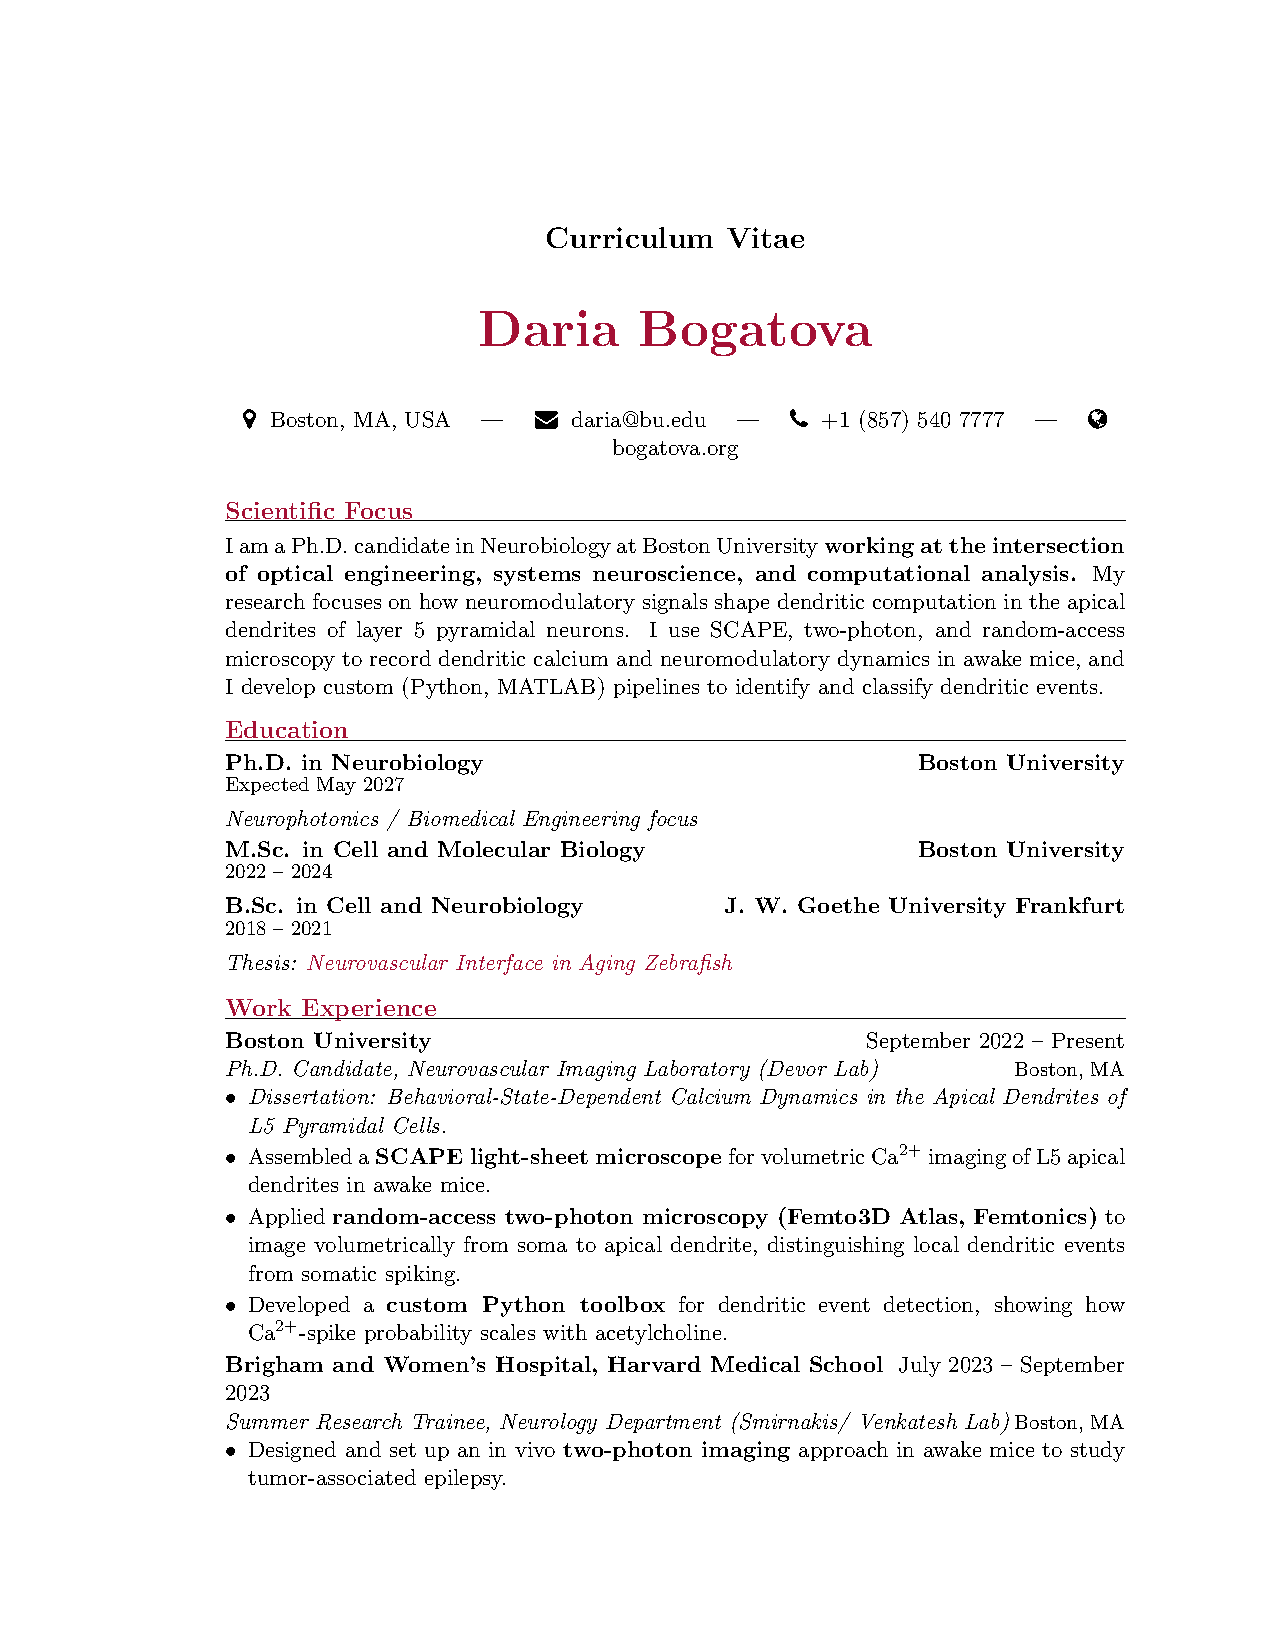
\includepdf[
	pages         = -,
	pagecommand   = {\thispagestyle{myheadings}},
	fitpaper      = false,
	offset        = 0 0
]{graphics/cv.pdf}


\end{document}
"
% or simply define \finaldraft at the top of main.tex.
%
% Check for leftovers before submitting:
%     grep -rn "needsinput" document/sections
\ifdefined\finaldraft%
	\newcommand{\needsinput}[1]{}
\else
	\newcommand{\needsinput}[1]{%
		\par\medskip\noindent
		\begingroup
			\small\sffamily\color{DarkRed}%
			\begin{singlespace}%
				\textbf{[NEEDS INPUT]}\quad #1%
			\end{singlespace}%
		\endgroup
		\par\medskip
	}
\fi

% -------------------------------------------------------------- shortcuts ---
% Statistics shorthands, so reporting stays consistent across chapters.
\newcommand{\pval}[1]{\ensuremath{p = #1}}
\newcommand{\pless}[1]{\ensuremath{p < #1}}
\newcommand{\mean}[2]{\ensuremath{#1 \pm #2}}
\newcommand{\nanimals}[1]{\ensuremath{n = #1}}

% Common italicised terms -- keeps species and gene names typeset correctly.
\newcommand{\invivo}{\emph{in vivo}}
\newcommand{\invitro}{\emph{in vitro}}
\newcommand{\exvivo}{\emph{ex vivo}}
\newcommand{\etal}{\emph{et al.}}

% Software names. Plain macros rather than glossary entries so they are safe to
% use inside captions and headings.
\newcommand{\mavca}{MAVCA}
\newcommand{\napari}{\textsc{napari}}

% Full citation of your own publications, used in the Introduction.
\newcommand{\printpublication}[1]{\AtNextCite{\defcounter{maxnames}{99}}\fullcite{#1}}

% ---------------------------------------------------------- approval page ---
% \readerC{ordinal}{name}{official title}{institution or empty}
%
% Always renders a blank signature rule. The copy submitted to ProQuest must be
% UNSIGNED (BU guide 1.4.1); signatures are collected through DocuSign and
% GRS attaches the signed page after review.
%
% Takes FOUR arguments. buthesis.sty's underlying \reader takes a fifth for the
% signature, which is supplied here, so you never pass it yourself. An earlier
% five-argument version silently swallowed the following token whenever a reader
% line was written with only four -- hence the fixed arity.
%
% Leave the institution empty for BU faculty. BU guide 1.4.3: a reader is
% assumed to be BU faculty unless you name another institution.
\newcommand{\readerC}[4]{%
	\reader{#1}{#2}{#3}{#4}{\rule{0.75\textwidth}{0.1mm}}%
}
